\documentclass[twoside,12pt]{article}

\usepackage{lipsum} % Package to generate dummy text throughout this template

\usepackage[sc]{mathpazo} % Use the Palatino font
\usepackage[T1]{fontenc} % Use 8-bit encoding that has 256 glyphs
\linespread{1.05} % Line spacing - Palatino needs more space between lines
\usepackage{microtype} % Slightly tweak font spacing for aesthetics

\usepackage[hmarginratio=1:1,top=30mm,bottom=30mm,left=30mm,right=30mm, ]{geometry} % Document margins
\usepackage{multicol} % Used for the two-column layout of the document
\setlength\columnsep{10mm}
\usepackage[hang, small,labelfont=bf,up,textfont=it,up]{caption} % Custom captions under/above floats in tables or figures
\usepackage{booktabs} % Horizontal rules in tables
\usepackage{float} % Required for tables and figures in the multi-column environment - they need to be placed in specific locations with the [H] (e.g. \begin{table}[H])
\usepackage[hidelinks]{hyperref} % For hyperlinks in the PDF

\usepackage{lettrine} % The lettrine is the first enlarged letter at the beginning of the text
\usepackage{paralist} % Used for the compactitem environment which makes bullet points with less space between them

\usepackage{graphicx, float}

\usepackage{abstract} % Allows abstract customization
\renewcommand{\abstractnamefont}{\normalfont\bfseries} % Set the "Abstract" text to bold
\renewcommand{\abstracttextfont}{\normalfont\small\itshape} % Set the abstract itself to small italic text

\usepackage{titlesec} % Allows customization of titles
\renewcommand\thesection{\arabic{section}} % Roman numerals for the sections
\renewcommand\thesubsection{\Alph{subsection}} % Roman numerals for subsections
\titleformat{\section}[block]{\large\scshape\centering}{\thesection.}{1em}{} % Change the look of the section titles
\titleformat{\subsection}[block]{\large}{\thesubsection.}{1em}{} % Change the look of the section titles

\usepackage{fancyhdr} % Headers and footers
\pagestyle{fancy} % All pages have headers and footers
\fancyhead{} % Blank out the default header
\fancyfoot{} % Blank out the default footer
%\fancyhead[C]{$\bullet$ Naiad AUV $\bullet$ } % Custom header text
\fancyfoot[C]{\thepage , team Naiad} % Custom footer text

%----------------------------------------------------------------------------------------
%	TITLE SECTION
%----------------------------------------------------------------------------------------

\title{\vspace{-15mm}\fontsize{24pt}{10pt}\selectfont\textbf{Naiad AUV}} % Article title

\author{
\large
Weronica Kovala (project manager), \and Anette Hilmersson (hardware lead), \and Jonatan Scharff Willners (software lead), \and Carl Ahlberg, \and Lars Asplund, \and Hampus Carlsson, \and Lennie Carl\'{e}n Eriksson, \and Mikael Ekstr\"{o}m, \and Andreas Gustavsson, \and Joakim Gustafsson, \and Ande Hana, \and Branko Miloradovic, \and Martina \"{O}hlund\\[2mm] % Your name
%\normalsize M\"{a}lardalen University \\ % Your institution
\vspace{-5mm}
}
\date{}
\begin{document}
\maketitle
\thispagestyle{fancy}
\begin{abstract}
Naiad is an AUV, designed and built during the last two years at M\"{a}lardalen University. The university has participated in RoboSub since 2012, but Naiad is a completely new robot. Naiad is built with a mono-hull which is designed to make it as hydro dynamic as possible. Modularity has been one of the aims in the designing of mechanics, electronics and software. The electronics for Naiad is mainly built on campus and it has been designed to fit the purpose and the design of Naiad to get the system as compact and modular as possible. For software, the system has been built in Ada with the aim to make a robust and modular system. 
\end{abstract}
\begin{multicols*}{2}
\section{Introduction}
Naiad is an Autonomous Underwater Vehicle (AUV) designed and built almost completely by M.Sc students at M\"{a}lardalen University in V\"{a}ster\aa s, Sweden. The project started in 2013 and for the majority of the time the team has contained 18 students majoring in robotics and intelligent embedded systems. At the moment there are 8 M.Sc students, 3 PhD students and 2 seniors in the team. 

The group was divided into four sub-groups which were managed by a project manager, a hardware and a software lead. The hardware group was divided into two groups, mechanical and electronics. In a similar fashion, the software group was divided into two sub-groups, one software group and one for simulation and motion (Fig. \ref{hierarchy}).
\begin{figure}[H]
\begin{center}
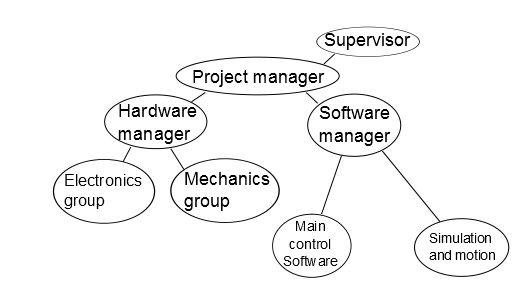
\includegraphics[width=0.4\textwidth]{./images/hierarchy.png}
\caption{The group was divided into four sub-groups, two for hardware and two for software.}
\label{hierarchy}
\end{center}
\end{figure}

Part of the task for the team has been to finance the project. The university provided around \$ 5000 for the project and the rest has come from sponsors. The low number of team members has made it impossible to let one person focus on marketing, which has created some difficulties when it comes to financing. 

The rest of this paper is structured as follows. In Section \ref{Hardware} the hardware, both mechanics and electronics, are described. In Section \ref{Software} the software system of Naiad is described. Section \ref{Future} describes the future works of the robot. 
\section{Hardware}
\label{Hardware}
The hardware of Naiad has been divided into two groups, mechanics and electronics. 
\subsection{Mechanics}
The main hull of Naiad has got a design which is made to be hydrodynamic and modular. Compared to previous designs from M\"{a}lardalen University this AUV is completely different, both in its design and its thruster configuration. Fig. \ref{Naiad} shows a CAD model of Naiad. All of the mechanics has been modeled in Solid Works. 

\begin{figure}[H]
\begin{center}
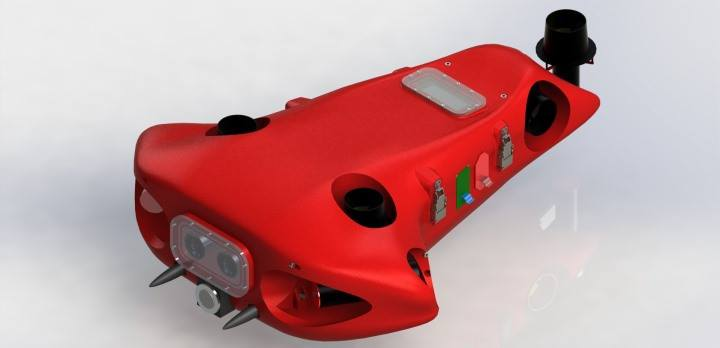
\includegraphics[width=0.4\textwidth]{./images/concept.jpg}
\caption{A concept image of the design of Naiad from Solid Works.}
\label{Naiad}
\end{center}
\end{figure}

Naiad's hull has been milled completely in the university and it is made out of polyurethane plastic, which was chosen due to the fact that it is easy to work with whilst still being hard and relatively cheap. An image of the finished hull can be seen in fig. \ref{first}. 

\begin{figure}[H]
\begin{center}
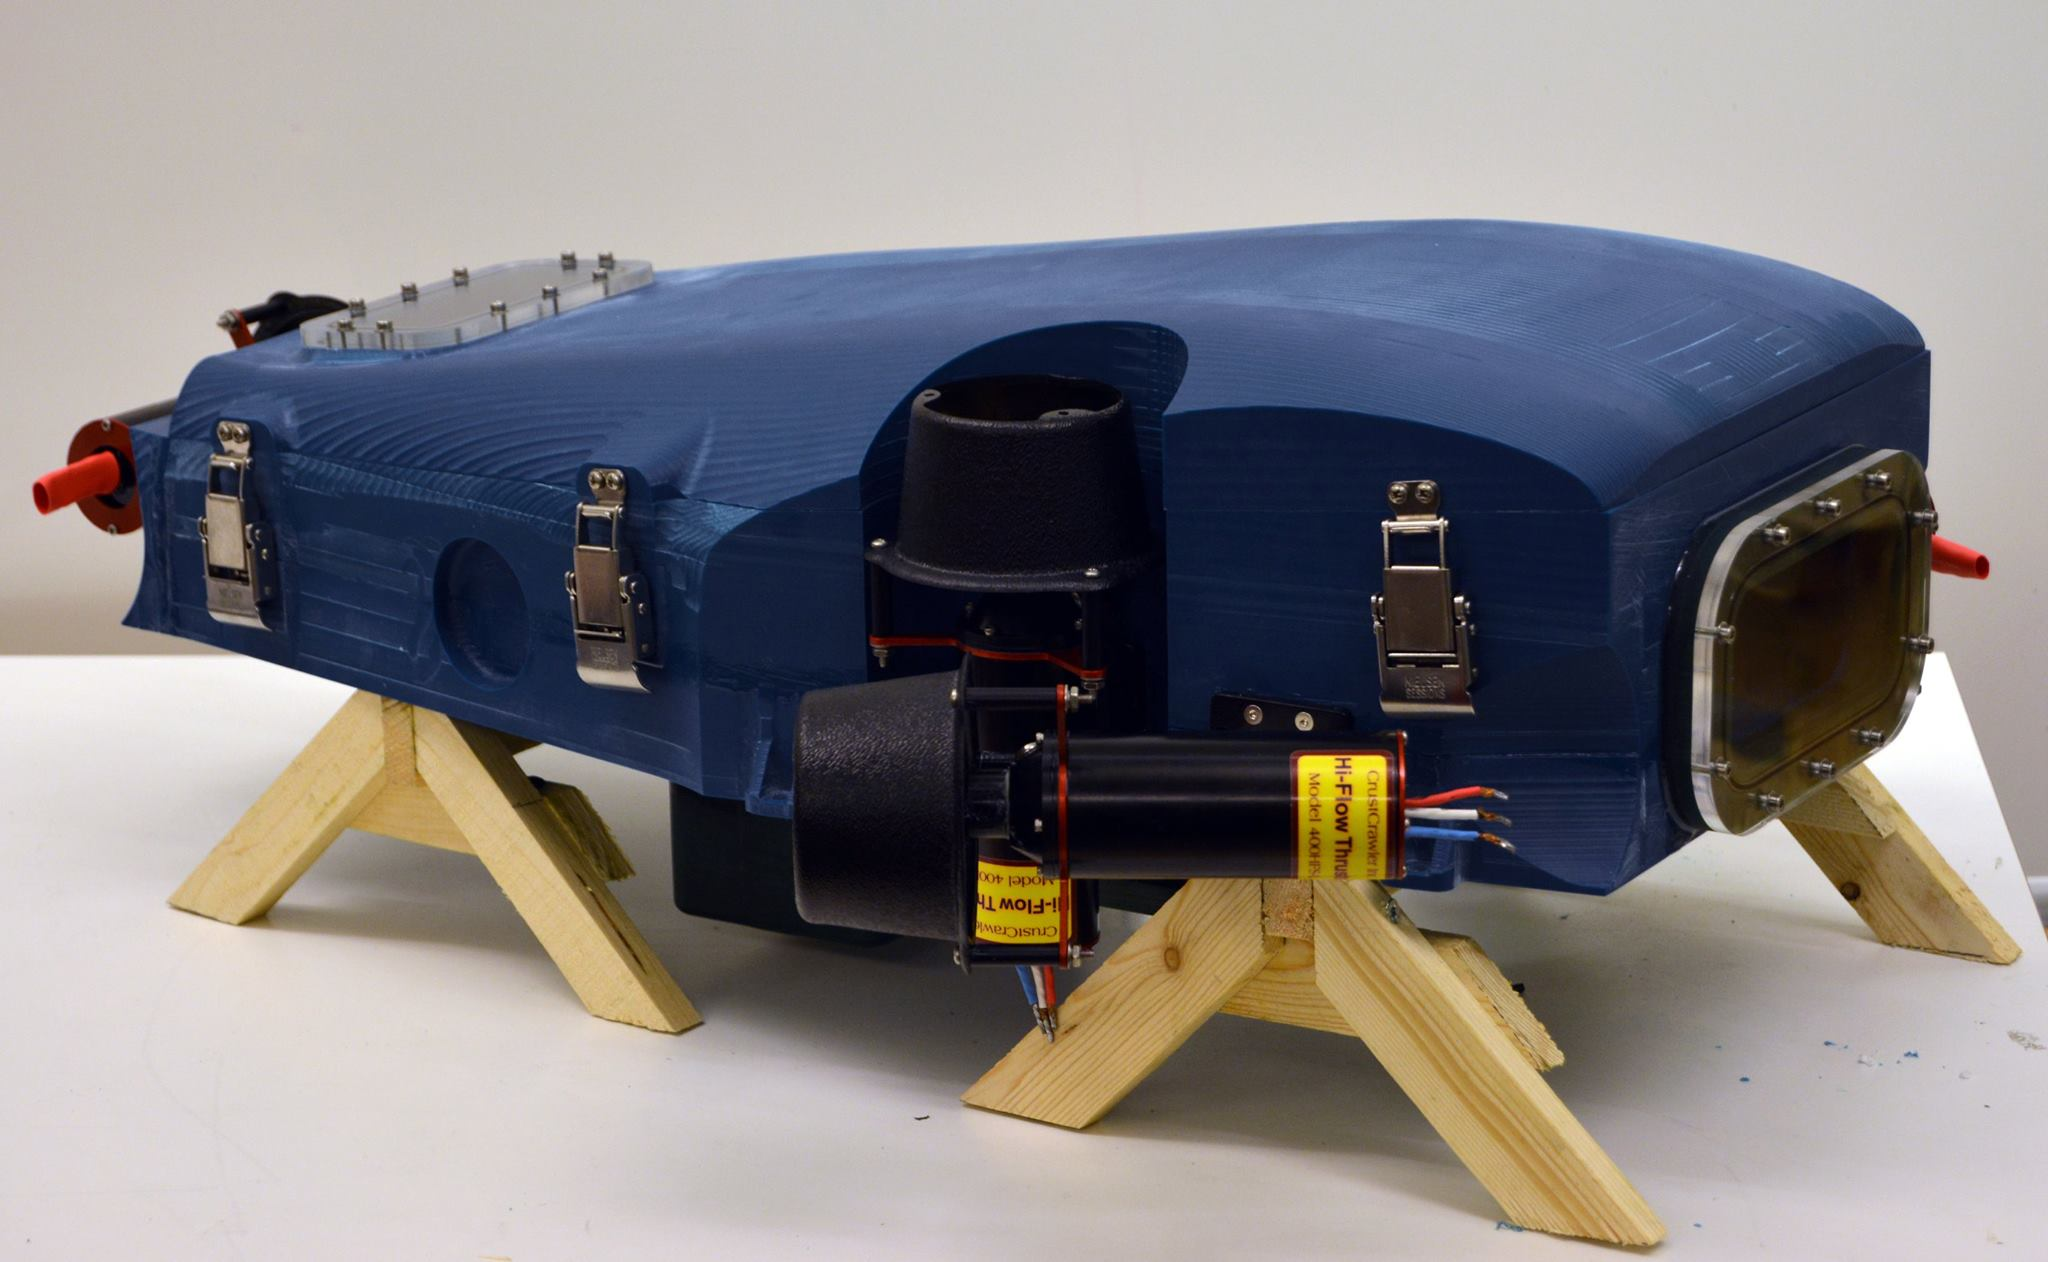
\includegraphics[width=0.4\textwidth]{./images/first.jpg}
\caption{One of the first images of the main hull when it was first put together.}
\label{first}
\end{center}
\end{figure}

\subsubsection{Thruster configuration}
The thrusters used on Naiad are Crustcrawler 400HFS thrusters. The thrusters are configurated using the configuration seen in figure \ref{thrusterconfig}. This type of configuration was chosen to make the AUV more agile and responsive than the configuration-type previously used in the university's AUVs. 
\begin{figure}[H]
\begin{center}
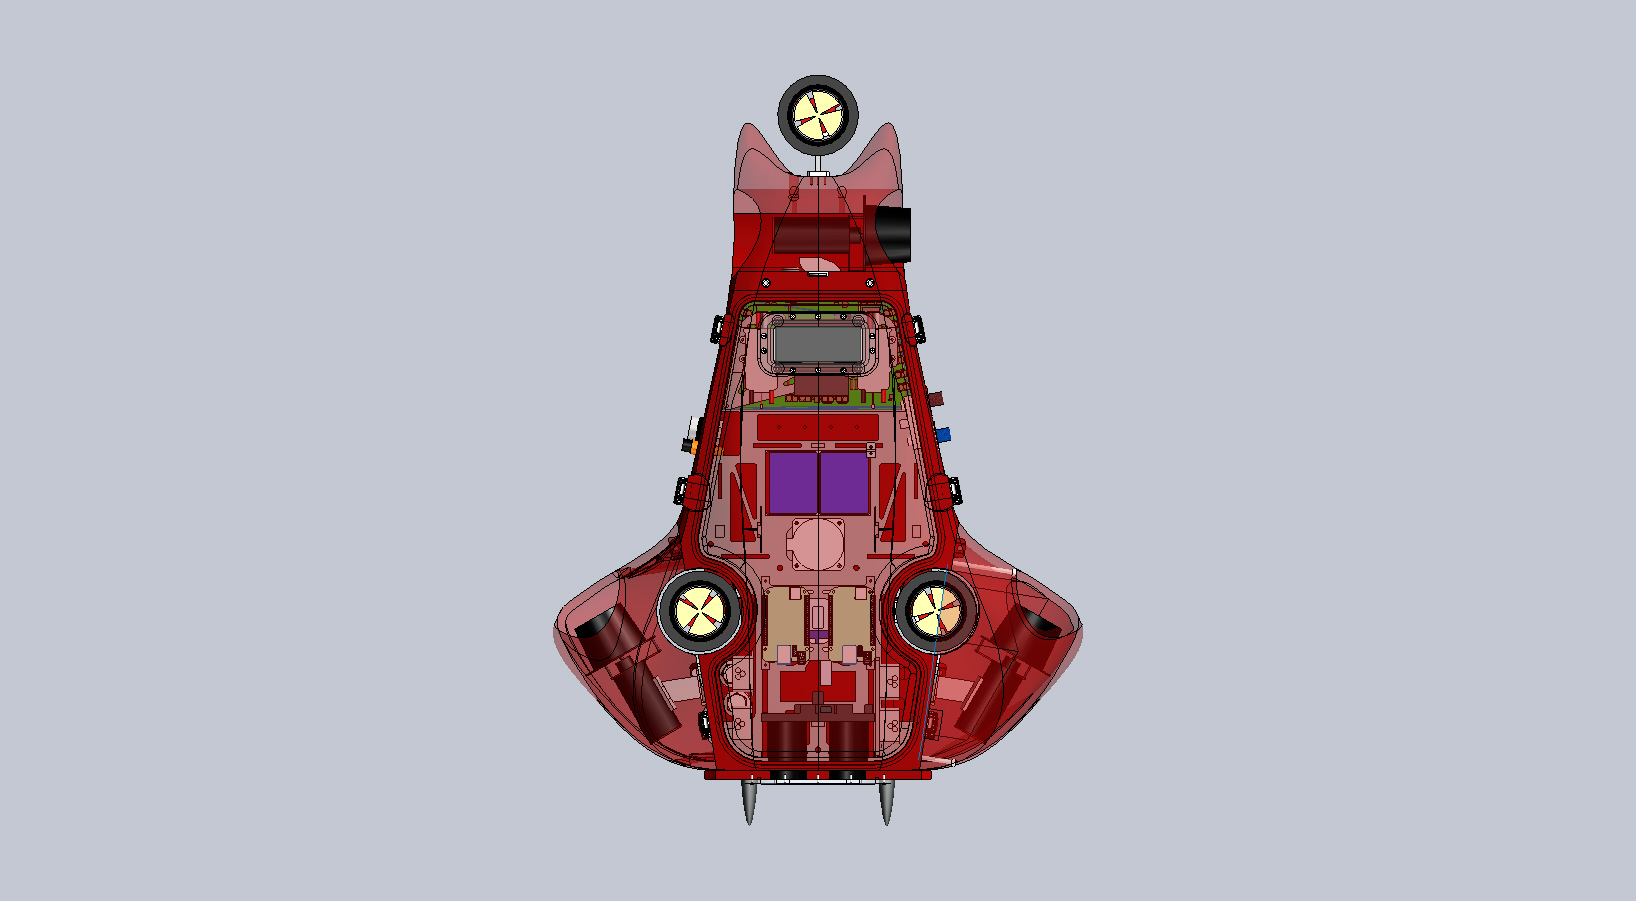
\includegraphics[width=0.4\textwidth]{./images/thcon.png}
\caption{The thruster configuration of Naiad.}
\label{thrusterconfig}
\end{center}
\end{figure}
The configuration enables 6 degrees of freedom (DOF). Three linear motions and three rotational motions. The linear motions are heaving (vertical movement), sway (side to side movement), surge (forward or backward motion). The three rotational motions are yaw (rotation around vertical axis), pitch (rotation around lateral, or side-to-side, axis) and roll (rotation around the longitudinal, or front/back, axis).

\subsubsection{Manipulator}
Naiad has a tendon driven manipulator that can be seen in fig. \ref{mani1}. The manipulator consists of two main parts, an arm which is able to bend in two places as well as rotate, and a hand. The hand has three fingers which can be used to grip a wide range of objects since it can achieve a cylindrical grasp, a circular grasp and a pinch/tip grasp (fig. \ref{grasps}). 
\begin{figure}[H]
\begin{center}
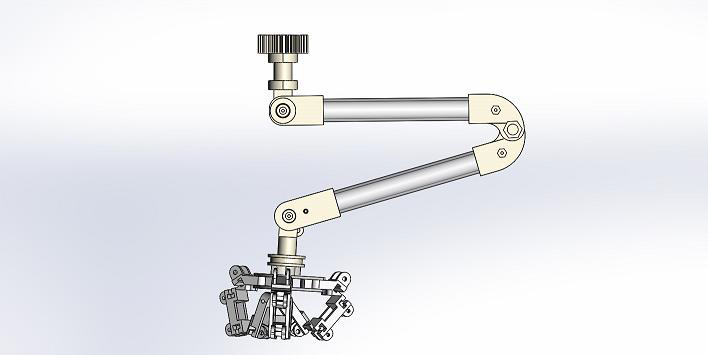
\includegraphics[width=0.4\textwidth]{./images/mani1.png}
\caption{CAD-figure of complete manipulator with both arm and hand.}
\label{mani1}
\end{center}
\end{figure}

\begin{figure}[H]
\begin{center}
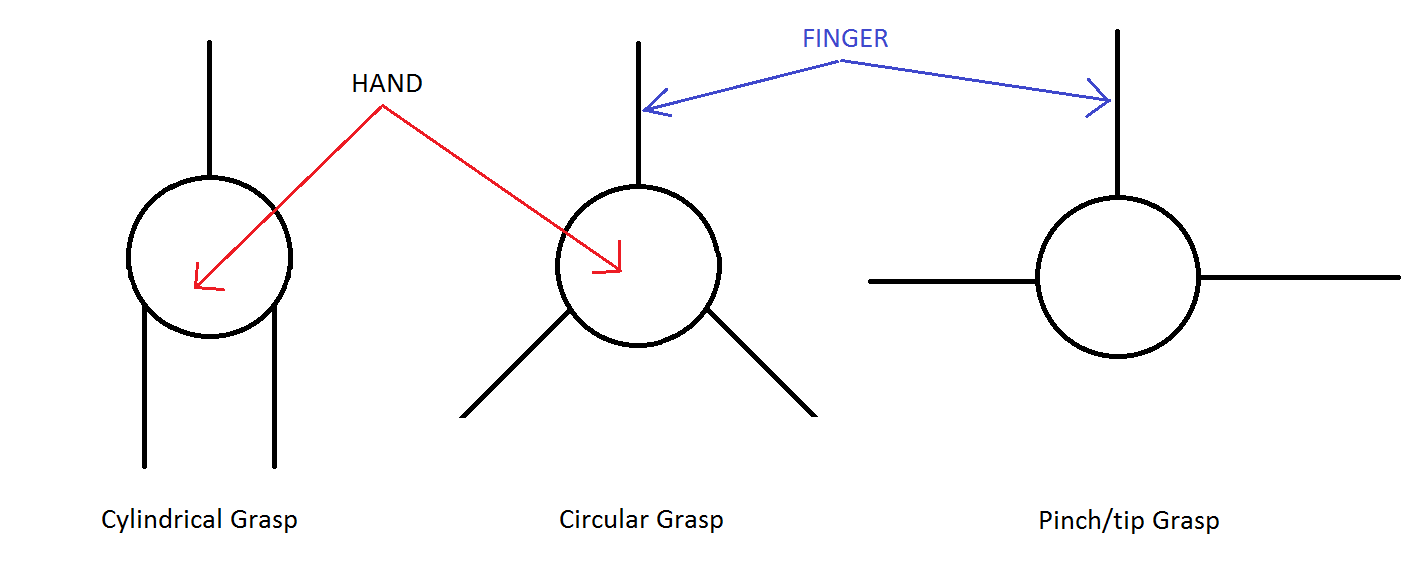
\includegraphics[width=0.4\textwidth]{./images/grasps.png}
\caption{The three different grasps the manipulator can use.}
\label{grasps}
\end{center}
\end{figure}

The hand on the manipulator is illustrated in fig. \ref{hand}. The gripper is naturally closed and has to be opened using a force, this ensures a stable grip. 
\begin{figure}[H]
\begin{center}
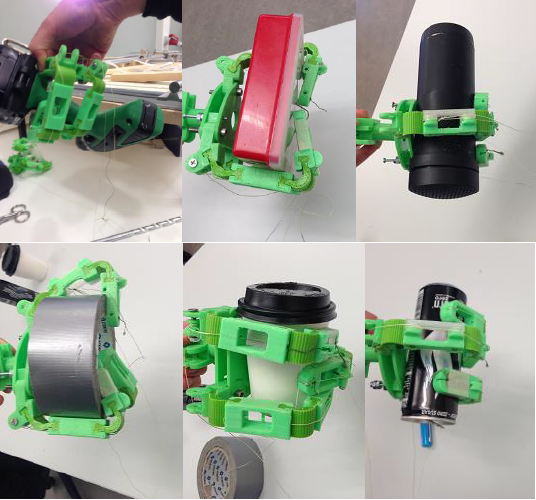
\includegraphics[width=0.4\textwidth]{./images/hand.png}
\caption{The final version of the tendon driven hand on Naiad in a variety of gripping positions.}
\label{hand}
\end{center}
\end{figure}
\subsubsection{Markers}
The markers are released using a solenoid. The main issue with the markers has been to get them heavy enough in order for them to drop in a straight enough line from the AUV down to the bottom of the pool. In order to get this 
to work, the marker, which is 3D-printed is fastened onto a bolt to increase the weight. The markers are mounted inside plexi-glass tubes close to the downward facing camera to improve aiming accuracy.
\subsection{Electronics}
The AUV is built with modularity as a key objective, therefore it is easy to add and remove different parts of the electronics. As much as possible has been developed on campus to ensure that the electronics will fit the purpose properly. This section has been divided according to the different types of electronics in Naiad, one section regarding the Power Supply Unit, another for the generic CAN-cards and one for the different extension boards that are present inside Naiad. 
\subsubsection{Power Supply Unit}
Naiad is powered using two 22,2 V Lithium Polymer (LiPo) batteries which are connected to the Power Supply Unit (PSU). The PSU is used to power the complete system. It converts the battery voltage to the different supply voltages. To control the supply to different parts of the system, a CAN-card is mounted on the PSU. To ensure safety, there is a hardware kill switch for the motors on this card which makes it possible to stop the power supply to the motors without shutting down the whole system. The kill switch is placed on the outside of the hull and short-circuits this connection to allow the motors to run using a magnet switch. 

Since the hull of Naiad is not squared in its shape, the PSU has been designed to fit the hull as closely as possible. The PSU is shown in fig. \ref{PSUcard} where it is mounted together with the CAN-card that is used to control the power supply to the rest of the system. 
\begin{figure}[H]
\begin{center}
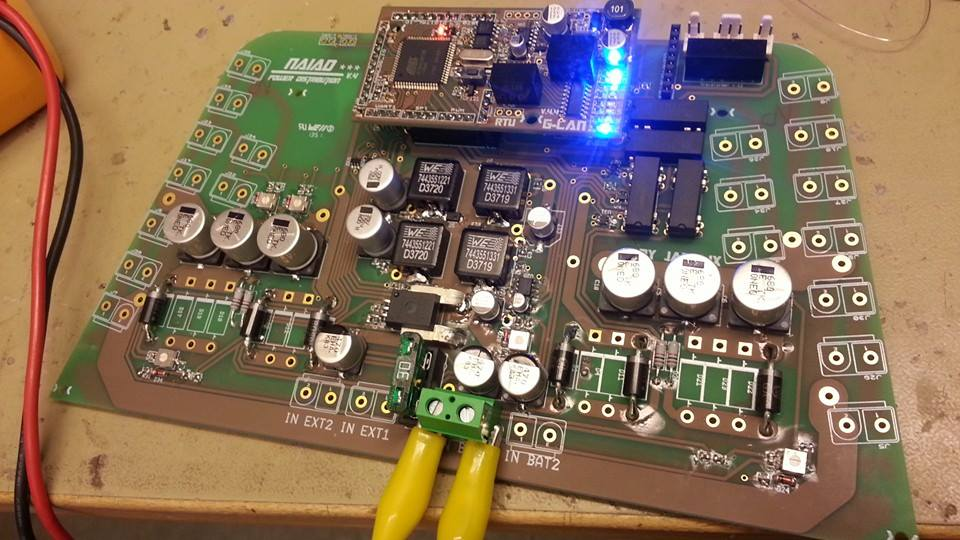
\includegraphics[width=0.4\textwidth]{./images/PSU.jpg}
\caption{The PSU with the CAN-card controlling the power supply to the rest of the system mounted for testing.}
\label{PSUcard}
\end{center}
\end{figure}
To monitor the system properly there are temperature sensors and current sensors on the PSU which make it possible to detect problems inside the hull and make the system act accordingly to add an extra dimension of safety and robustness to the system. 
\subsubsection{CAN-card}
A generic CAN-card has been created to form the base of the Controller Area Network (CAN) bus. The Microcontroller Unit (MCU) on these are the AT90CAN128. In order for the system to be modular the CAN-cards are placed in stacks using a pin header on the card and a socket header on the stacks which makes it possible to slide the cards into the socket header. In a similar fashion, there are extension boards to change the functions of the generic CAN-cards. For example there is an extension board for the motor signals, the sensor handling, and for the actuators. The CAN-card can be seen in fig. \ref{CANcard}.

\begin{figure}[H]
\begin{center}
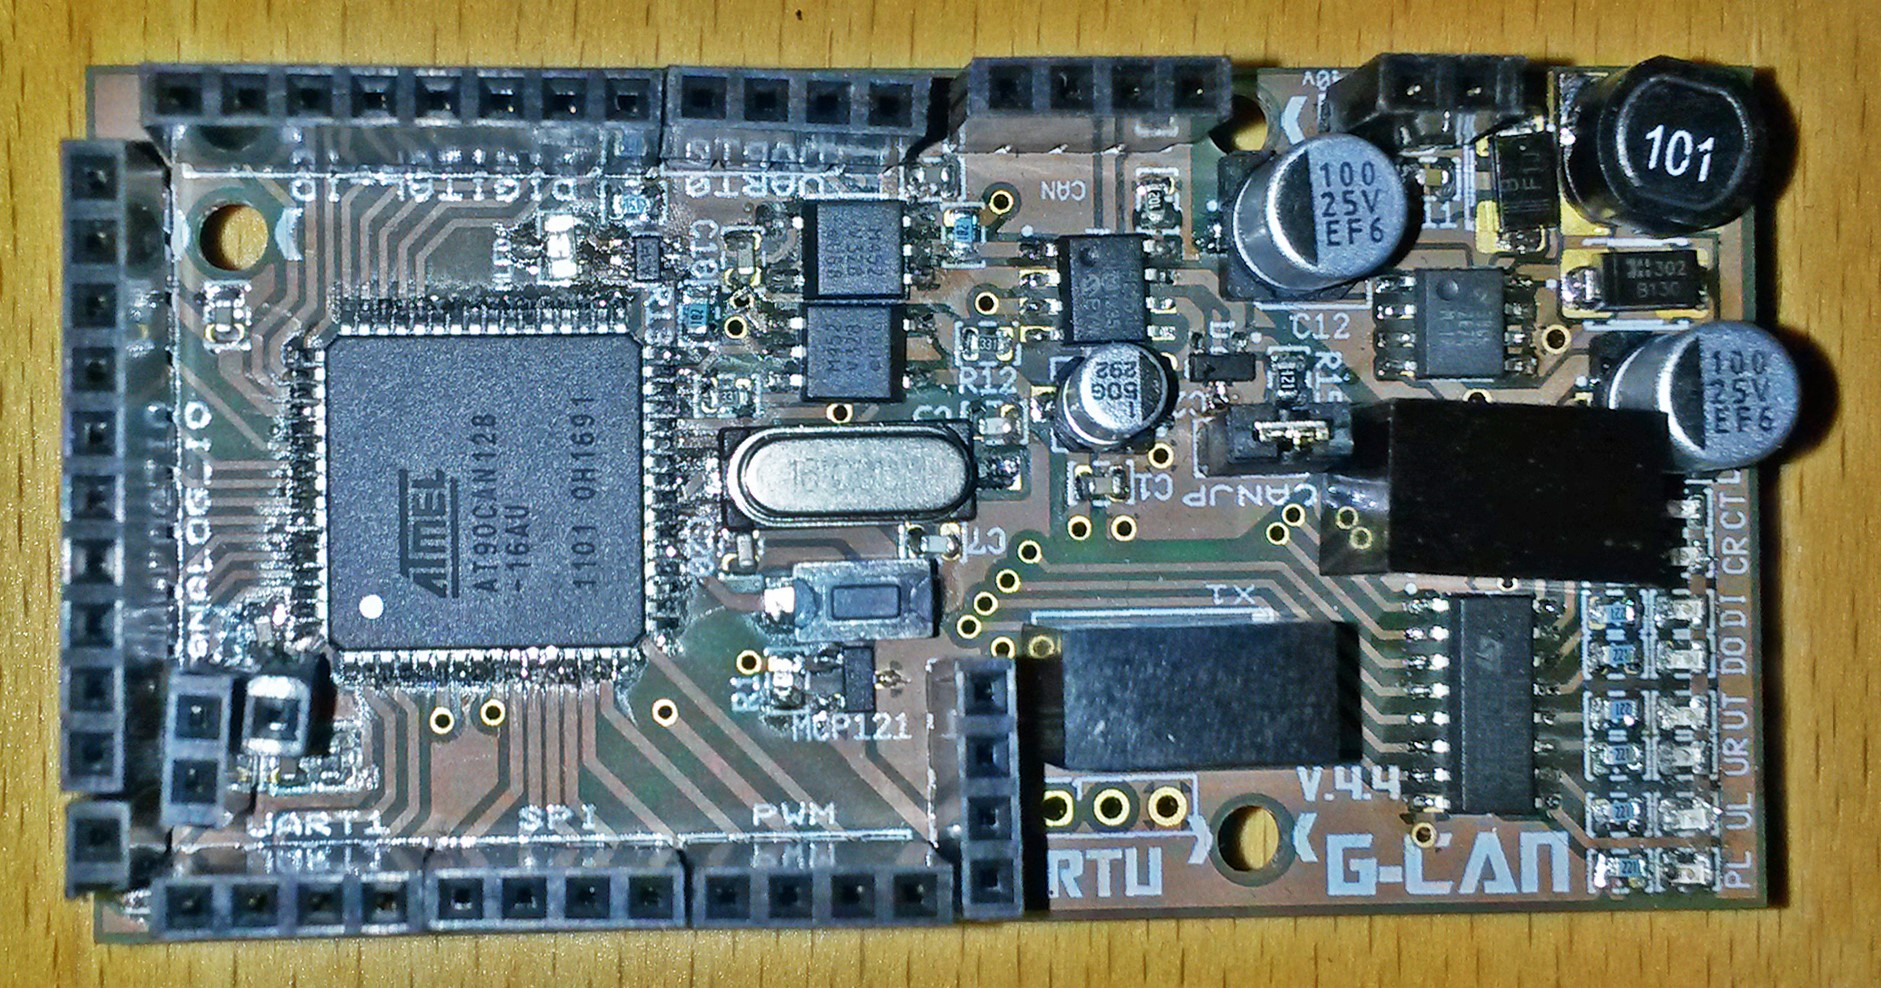
\includegraphics[width=0.4\textwidth]{./images/CAN.jpg}
\caption{The generic CAN-card.}
\label{CANcard}
\end{center}
\end{figure}

\subsubsection{Extension boards}
There are a number of extension boards in the electrical system of Naiad. 
\begin{itemize}
\item Motor extension - the thrusters are controlled using a Phoenix Ice2 HV 60 motor controllers used with the Castle Link V3.52.10 software. The signal to the motor controllers come from the motor extension board which provides the controllers with 5V and GND from the CAN-cards as well as a PWM-signal to each motor. One motor extension board can control all six motors on Naiad.
\item Sensor extension - the sensor extension board is used to transfer the sensor data from the sensors to the CAN-bus. At the moment the only sensor that uses this board is the pressure sensor.
\item Actuator extension - the actuator extension board is used to control the solenoid that releases the markers. It is also prepared for releasing torpedoes in a pneumatic system, which is yet to be implemented. 
\item INS extension - the INS board contains the electronics to get the measured data from the Inertial Measurement Unit (IMU) through a UART interface. It is also able to transfer the data from the Fiber Optical Gyroscope (FOG) to the CAN-card using a SPI-interface. 
\end{itemize}

\section{Software}
\label{Software}
The software section has been divided into three parts, one for the main control which handles motion and internal communication in Naiad, another section for the vision system and a third section regarding the simulator. 
\subsection{Main control}
The main computer on Naiad is a Beagle Bone Black (BBB) where, both on this card and on the CAN-cards, all code is written in Ada taking Ravenscar into consideration. All of the node to node communication is based on either CAN or Transmission Control Protocol (TCP) where the former is communication between CAN-cards. The latter is between nodes that are either on a BBB, a GIMME-2 card or other nodes that are connected via Ethernet. A node on the CAN-bus is still able to communicate with a node on a BBB by passing through a translation node.

A node can choose what type of values to subscribe to by sending a message containing this information to the routing node. When a node sends data to the routing node, the data will be distributed to all nodes that needs this information. With this approach, the system and nodes do not need to be changed when implementing a new node/task. This leads to starting a new node for the first time can be implemented when the code for that node is completed, reducing development time for new functions.

With all communication going through a central node, and no direct communication, there will be an overhead, but with small messages the benefit of this modular system outweighs this drawback. An other advantage of this type of system is safety, in a safety-critical system such as a robot, a node dying can cause the whole system to fail, with a central node keeping track of all nodes still being alive this problem can be found and solved. A flow-chart of the node communication in the system can be seen in fig. \ref{softwareflow}.

To control the motion of Naiad, one Proportional Integration Derivative (PID) and five Proportional Derivative (PD) controllers were used. The PD/PID controller bases its control values on the difference (error) between the desired and the current state of the robot. 

To determine the position of the AUV, the accelerometer data from the IMU are integrated twice. However, there is a lot of noise on this signal and when the signal is integrated, the noise increases. To reduce the noise a Kalman filter is used. 

\begin{figure}[H]
\begin{center}
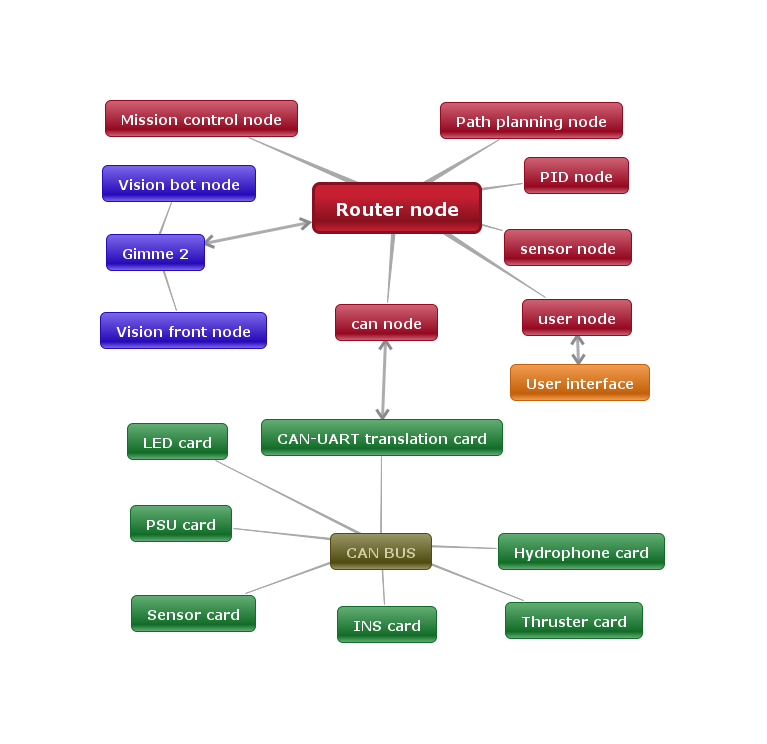
\includegraphics[width=0.4\textwidth]{./images/flowchart.png}
\caption{Flowchart of the complete software system}
\label{softwareflow}
\end{center}
\end{figure}

\subsection{Vision}
There are two stereo vision camera systems on Naiad, one that is facing forward and one downwards, which can be seen in fig. \ref{cameras}. 
\begin{figure}[H]
\begin{center}
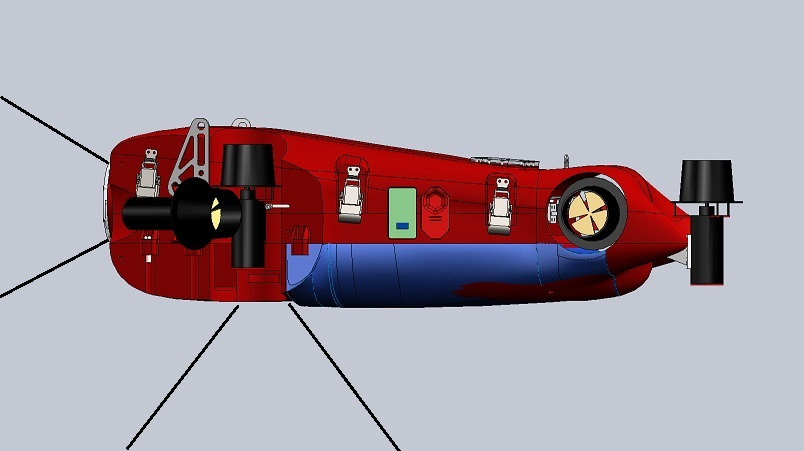
\includegraphics[width=0.4\textwidth]{./images/cameraplacement.jpg}
\caption{Illustration of the placement of both stereo vision systems.}
\label{cameras}
\end{center}
\end{figure}
The vision-system in Naiad are two GIMME-2 stereo-vision boards. The processor on these boards is a zynq processor which has an ARM Cortex A9 dual-core processor combined with an FPGA in the same chip, which enabled some of the vision to be done directly on an FPGA, which makes the processing fast. There are two 10 megapixel image sensors on each GIMME-2 board. Since the image processing is done on the GIMME-2 board, the system for front and downward vision are completely separated. The OpenCV library is used for image processing, which significantly reduces software development time. In order to make the use of OpenCV easier, the code for the vision system is written in C/C++.

The images are analysed directly on the boards and the relevant information is sent to the router node in the system. Relevant information is for example information about distance and angle towards the object. 
\subsection{Simulation}
The simulator for Naiad has two modes, either simulation or IMU mode. In simulation mode a virtual simulated representation of the Naiad robot is run with simulated sensors and actuators. The simulation allows you to be connected directly to the PID controller through TCP sockets, sending equal data as the real sensor node would have done if the robot was running a real task and receiving the real motor values that the PID controller would send to the real robot. These motor values are turned into estimated forces that is shown as dynamic lines coming from the different motor positions to give a good visualization of the forces that is acting on the robot. An illustration of the simulation can be found in fig. \ref{simulation}.
\begin{figure}[H]
\begin{center}
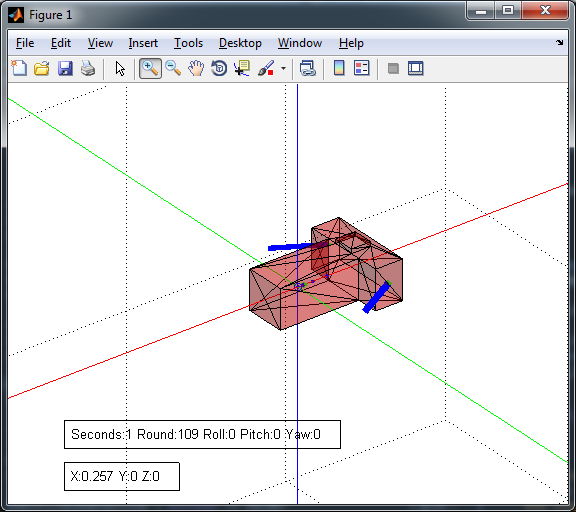
\includegraphics[width=0.4\textwidth]{./images/simforward.png}
\caption{Concept image from the simulation environment.}
\label{simulation}
\end{center}
\end{figure}
In IMU mode the simulator can be set into a passive mode that shows a virtual visual representation
of the estimated position and orientation that the system in real time has estimated. No calculations
is needed in this mode more than rotating the virtual robot in the right order.
\section{Strategy and current status}
\label{Future}
With about one month left for the competition the main issue is to get the object detection to work properly. The robot is able to move properly on command but without vision it is hard to know where to move. Therefor this is the main issue at this point. 

The markers and the manipulator are yet not attached to the hull, which is a concern for the team. The aim for the mechanics group is, at this point, to try getting these finished in the time left before the competition. The first aim is to get the missions that does not need these features. 

Since the university does not have a pool on its own the public pool has been used, which made testing harder since it becomes an all day task for almost the entire team to move everything there, do the testing and then moving everything back. A smaller garden pool which is 5 m wide has also been available on campus. This pool has two major limitations; since it is placed outside it is not possible to use it during the winter and its size makes it impossible to use it for testing full missions. 
\section{Acknowledgements}
We would like to thank everyone, both faculty and others, who has helped the team with the development of Naiad; Emil Bergstr\"{o}m, Nils Brynedal Ignell, Cezar Chiru, Gerard Duff, Fredrik Ekstrand, Martin Ekstr\"{o}m, Simon Elgland, Christoffer Holmstedt, Omar Jamal, Konstantin​os Konstantop​oulos, Joel Larsson, Daniel Lindqvist, Johan Mattsson, Michael Mayer, Per-Erik M\aa hl, Nahro Nadir, Debajyoti Nag, Niclas Rasmusson, Aseem Rastogi, Patrik P\"{a}rlefjord, Rizwin Shooja, Wenkai Wang. And our sponsors; \\
\textbf{Level 1:} W\"{u}rth Elektronik \\
\textbf{Level 2:} Robotdalen, FoU R\aa det, Deepvision \\
\textbf{Level 3:} Kvaser, Packsize
%\section{Bibliography}
%\bibliographystyle{IEEEtran}
%\bibliography{journal}
\end{multicols*}
\end{document}
